\documentclass{article}
\usepackage[T1]{fontenc}
\usepackage{lmodern}
\usepackage{graphicx}
\usepackage{amsmath,amssymb}
\usepackage[a4paper,margin=2cm]{geometry}
\usepackage[absolute,overlay]{textpos}
\setlength{\TPHorizModule}{1mm}
\setlength{\TPVertModule}{1mm}
\usepackage[indonesian]{babel}
\usepackage{hyperref}
\setlength{\emergencystretch}{2em}
% unit: Halaman 43

\begin{document}

% === Halaman 43 (llm) ===

\begin{center}
\Huge Dua Aplikasi Utama Enkripsi
\end{center}

\begin{itemize}
    \item Enkripsi dokumen di dalam storage (\textit{encryption at rest})
    \item Enkripsi pesan yang dikirim (\textit{encryption on motion})
\end{itemize}

\vspace{70mm}

Sumber: \url{https://www.scienceabc.com/innovation/how-whatsapp-app-message-end-to-end-encryption-works-msgs-security-method-key.html}

% deskripsi: Screenshot jendela dialog 'Encrypt Document' yang menampilkan kolom input password dan peringatan tentang kehilangan password.
% bbox normalisasi: [0.0500, 0.4400, 0.4600, 0.8800]
\begin{textblock*}{86.10mm}(10.50mm,130.68mm)
\noindent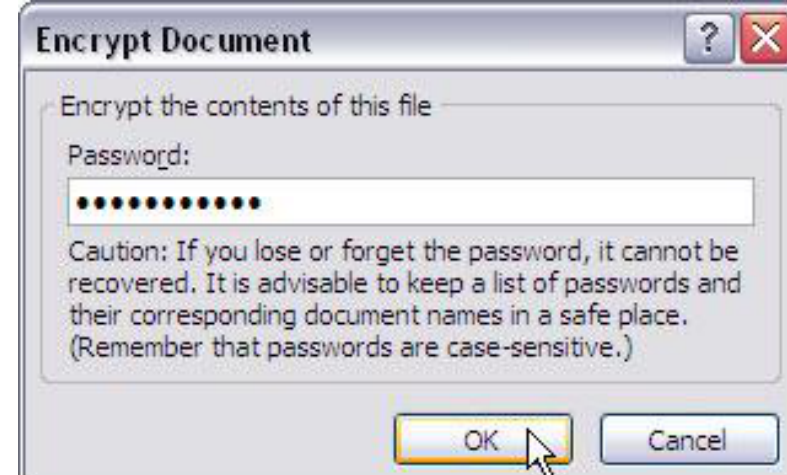
\includegraphics[width=86.10mm,height=130.68mm]{../../images/llm/page_043_img_01.png}%
\end{textblock*}

% deskripsi: Foto layar smartphone yang menampilkan percakapan WhatsApp dengan notifikasi bahwa pesan diamankan dengan enkripsi end-to-end.
% bbox normalisasi: [0.5300, 0.4300, 0.9100, 0.8800]
\begin{textblock*}{79.80mm}(111.30mm,127.71mm)
\noindent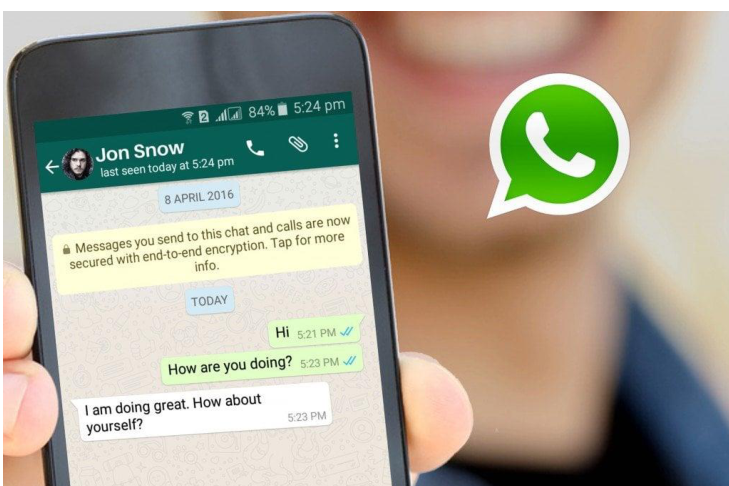
\includegraphics[width=79.80mm,height=133.65mm]{../../images/llm/page_043_img_02.png}%
\end{textblock*}

\end{document}
